\section{方法}\label{sec:method}

\subsection{任务定义}\label{sec:task}
本文聚焦农业机器人最常见的前向作业视野：输入正前、左前和右前三路相机，预测前方 $20\,$m 的三维语义占用。
给定时刻 $t$ 的三路同步图像 $\I_t=\{I_t^{\mathrm{FL}},I_t^{\mathrm{F}},I_t^{\mathrm{FR}}\}$、
相机内外参和机器人坐标系，目标是在前向空间
\begin{equation}
\B=[0,20]\times[-10,10]\times[-2,3]~\mathrm{m}
\end{equation}
中预测语义占用。体素分辨率为 $0.2~\mathrm{m}$，因此输出网格为 $100\times100\times25$。
每个有效体素 $v\in\V$ 的标签 $y_v\in\{0,\ldots,5\}$ 分别表示自由空间、
作物、土壤地面、道路、其他植被与其他障碍物。

\subsection{AgriOcc-Dataset 构建}\label{sec:dataset_construction}
AgriOcc-Dataset 基于 Unreal Engine 5 的 FarmSim 环境构建，面向农业机器人前向作业时的多视角三维语义占用感知。每个序列包含六路同步 RGB 图像、相机内外参、机器人位姿、语义占用标签及有效体素掩码；本文的主任务从中选取正前、左前和右前三路图像。标签在加载阶段统一映射为 free、crop、soil\_ground、drivable、other\_vegetation 和 other\_obstacle 六类，并在机器人自身坐标系中生成前方体素监督。

数据集包含 298 个完整序列和 38,862 帧，其中 248 个序列（32,385 帧）用于训练，50 个序列（6,477 帧）用于验证；划分以完整序列为单位，以避免同一路径或相邻帧同时出现在训练和验证集中。数据覆盖 cabbage、carrot、corn、cucumber、potato、radish、redbeet、sunflower、tomato 和 wheat 十种作物；每种作物进一步包含 early、mid 和 mature 三个生长阶段，并覆盖 dawn、morning、noon、evening 和 night 五个时段，以及 cloudy 与 sunny 两类天气。图\ref{fig:crop_distribution}给出了总体数据集的作物组成，potato 和 tomato 各占 14.09\%，cucumber 占 2.01\%，其余类别占比介于 6.04\% 与 12.08\% 之间。

\begin{figure}[t]
\centering

\includegraphics[width=0.88\linewidth]{figures/crop_distribution.pdf}
\caption{AgriOcc-Dataset 中 298 个完整序列的作物组成。扇区面积表示各作物的序列占比，标注给出作物名称、序列数与百分比。}
\label{fig:crop_distribution}
\end{figure}

\subsection{AgriOcc 总体结构}\label{sec:architecture}

图\ref{fig:overview}给出 AgriOcc的总体架构。
图像编码器使用 ImageNet/FCOS3D 预训练的 ResNet-101 与 FPN 提取四级二维特征。
随后，六层 GeoVis-BEV 编码器以 GVAD 作为 BEV token 的上下文增强单元：在每个编码层内，
GVAD 先结合局部可变形更新与可见性引导的全局锚点，为当前 BEV 查询补充可靠的空间上下文；
再由空间交叉注意力依据相机投影关系，从多尺度图像中聚合几何对齐的视觉证据。
经逐层更新后，编码器输出 $100\times100$、通道数为 256 的 BEV token；
三层占用解码器提供多层监督，其中最后一层由 Agri-AMoE 将 BEV token 提升为
三维特征体并预测 25 个高度位置上的六类 logits。
因此，AgriOcc 利用 GVAD 优化 BEV 编码过程中的可见性驱动全局上下文建模，以 Agri-AMoE 自适应建模三维局部结构，
并以近远场布局将早期编码计算聚焦于近场精细结构。

\begin{figure}[t]
\centering
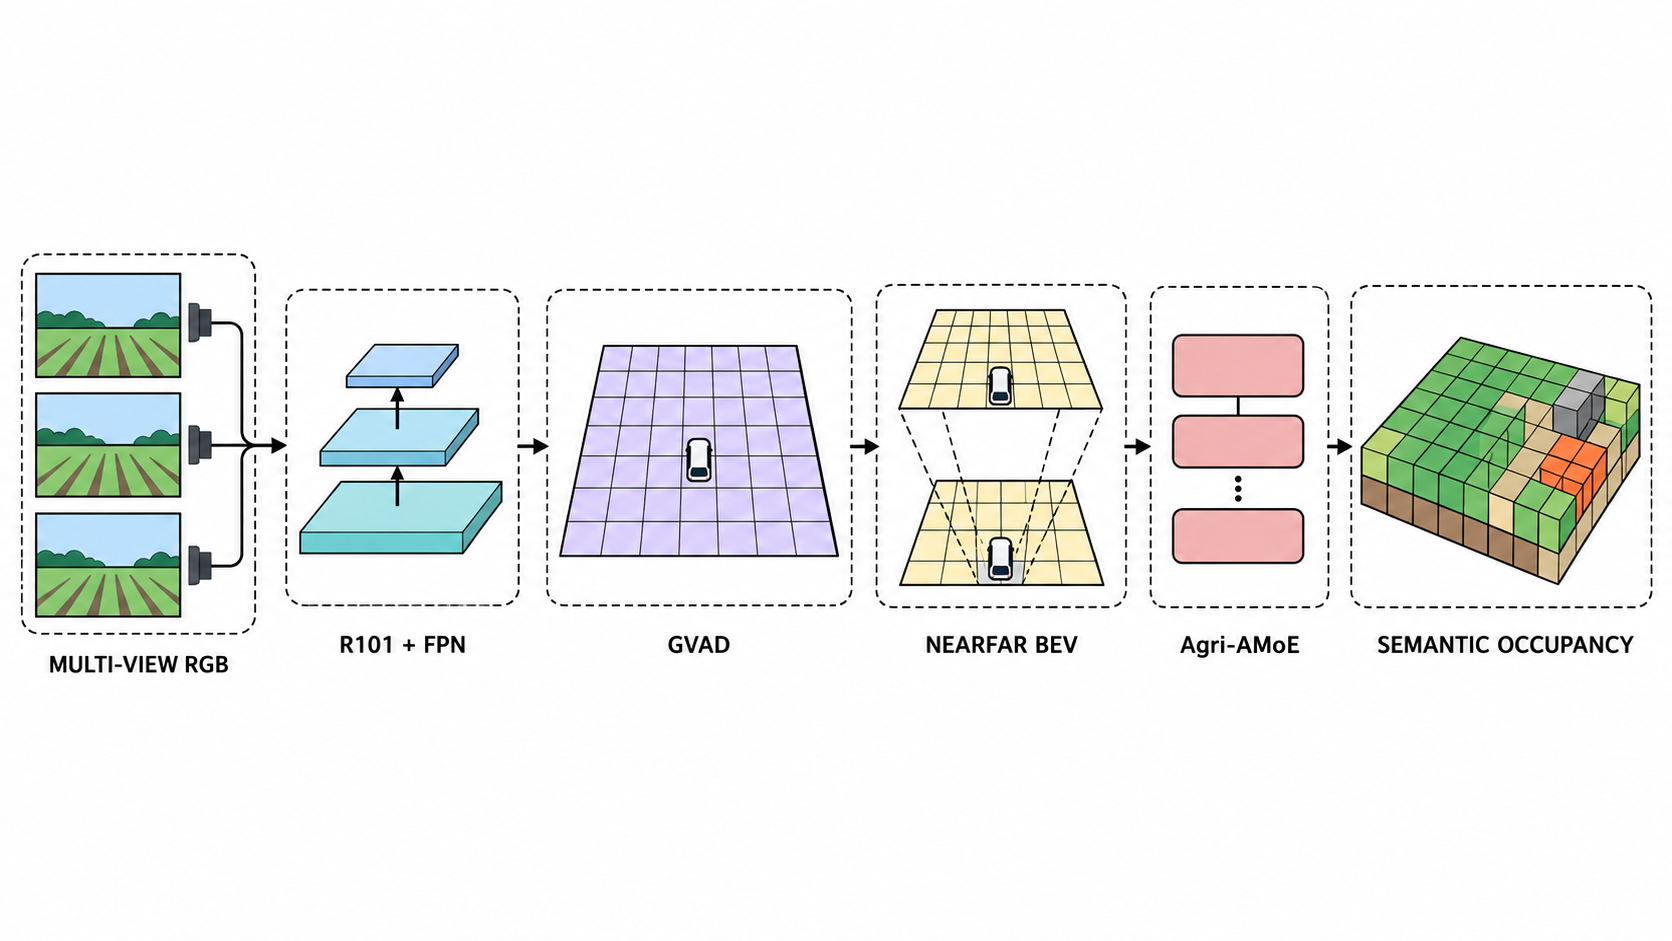
\includegraphics[width=\linewidth]{figures/agriocc_overview_imagegen.png}
\caption{AgriOcc 总体结构。三路前视图像经 ResNet--FPN 提取多尺度特征；GeoVis-BEV 编码器将多相机证据聚合至前方鸟瞰空间；近远场布局优先分配近场计算；最后一层占用解码器通过 Agri-AMoE 将 BEV token 提升为三维体积，并输出 $100\times100\times25\times6$ 语义 logits。}
\label{fig:overview}
\end{figure}

\subsection{GeoVis-BEV 编码器}\label{sec:bev-encoder}

本文将几何关系与观测可见性协同建模的编码过程称为 GeoVis-BEV 编码器（Geometry- and Visibility-aware BEV Encoder）。
该编码器承接图像编码器输出的多尺度特征，并将其逐层汇聚为用于占用预测的鸟瞰表征。
对第 $l$ 层输入的 BEV token，编码器首先利用 GVAD 强化局部结构与可靠的长程上下文，
再结合相机投影关系聚合图像条件特征，并通过前馈网络完成表征更新。
这一过程在六个编码层中重复执行，输出保持为 $100\times100$、通道数为 256 的稠密 BEV token。
此外，近远场查询布局在编码早期优先保留近场的高分辨率 token，
使计算分配与农业作业场景中的空间重要性相匹配。

\begin{figure}[t]
\centering
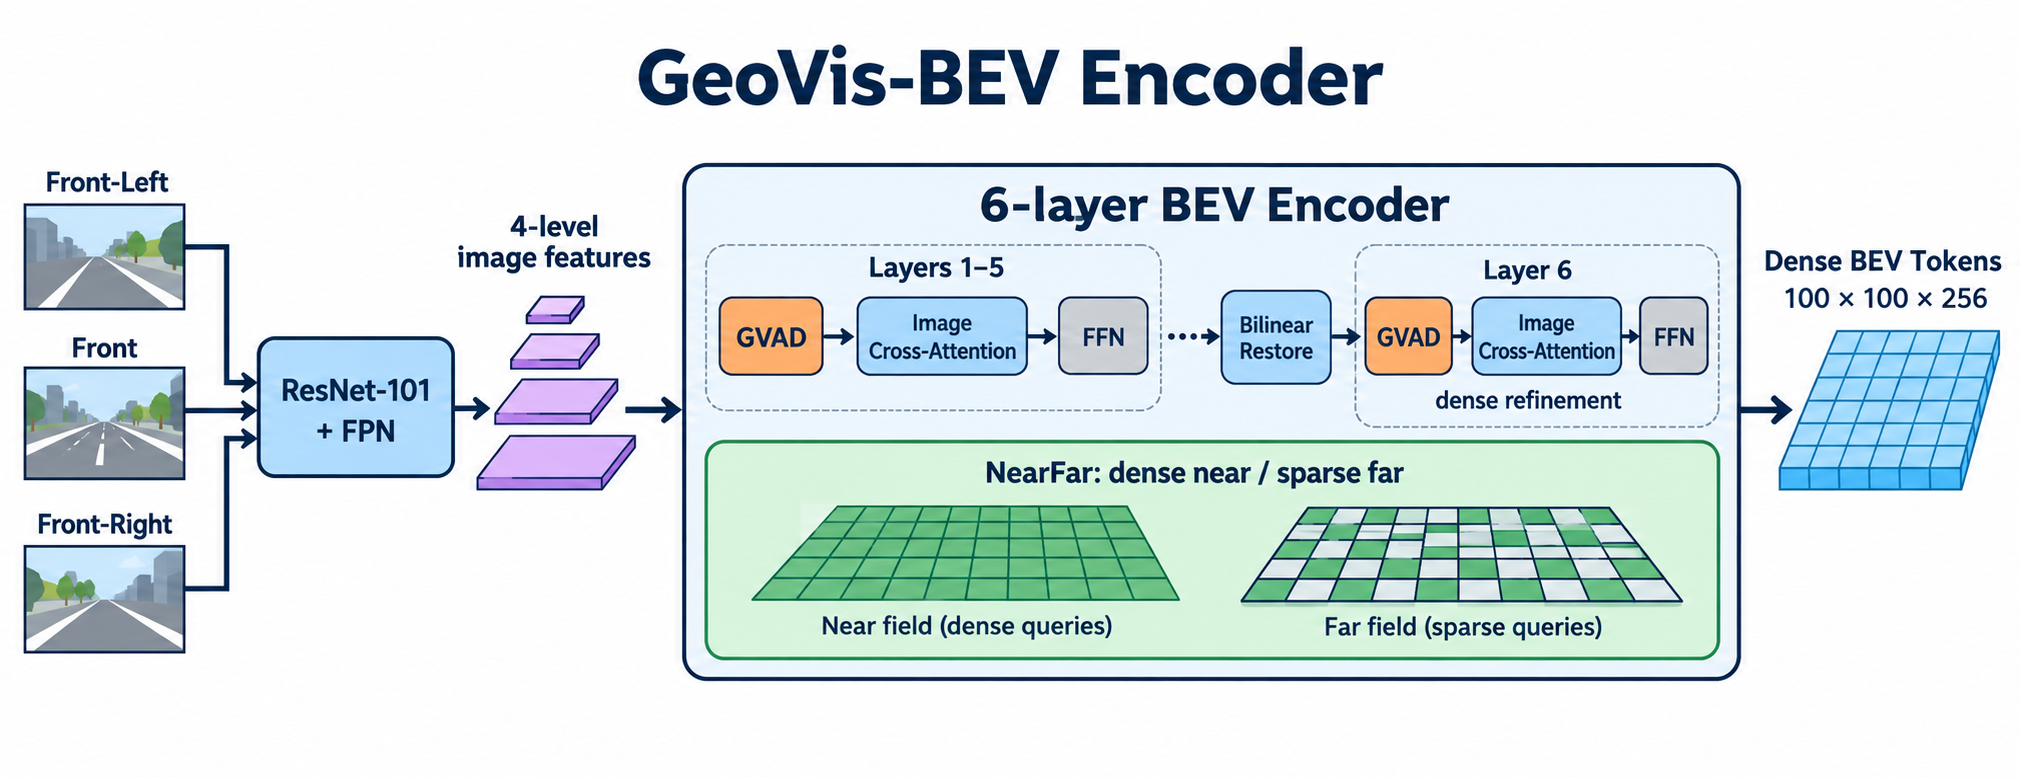
\includegraphics[width=\linewidth]{figures/geovis_bev_encoder_overview.png}
\caption{(a) GeoVis-BEV 编码器整体架构。三路前视图像经 ResNet--FPN 提取多尺度特征后输入六层编码器；GVAD 在各编码层中更新 BEV token，NearFar 在前五层保留近场稠密查询并对远场规则稀疏采样，恢复为稠密网格后由最后一层完成图像条件细化。}
\label{fig:geovis-bev-encoder}
\end{figure}

\subsubsection{几何可见锚点可变形注意力}\label{sec:gvad}
农业机器人依靠RGB摄像头观测作业区域时，作物冠层遮挡、
视场边缘截断与重复纹理会使部分 BEV 单元缺少直接、可靠的投影证据。
尤其在作物行内部，局部图像特征容易将叶片、垄沟和株间空隙混淆；
若只依赖局部采样，弱可见单元难以从同一行或相邻行的连续结构中获得补偿。
反之，通用的全局上下文聚合通常对所有区域一视同仁，可能将低置信观测传播至本应保持精细边界的区域。
因此，BEV 编码器需要同时保留几何对齐的局部细节，并根据每个单元的实际可见性，有选择地从可靠区域读取长程上下文。

为此，本文在多层 BEV 编码器中引入几何可见锚点可变形注意力（GVAD），
用于在每层的图像条件特征聚合前增强 BEV 查询。局部可变形采样与 Deformable DETR\cite{zhu2021deformable}
的稀疏参考点聚合、以及 DETR3D\cite{wang2022detr3d} 的三维查询投影机制一脉相承，
但后两者对观测可靠性的利用仍是隐式的。GVAD 在保持 BEV token 输入输出尺寸不变的前提下，
将局部可变形路径与可见性加权的全局锚点路径耦合，使弱可见单元获得可靠上下文，
同时使直接可见区域仍以局部投影证据为主。由此，GVAD 不是独立的占用预测头，
而是服务于逐层 BEV 表征更新的编码组件。

设第 $l$ 层的 BEV token 为 $\bm{q}_i\in\R^d$，由相机投影有效掩码得到其可见性 $m_i\in[0,1]$。
将 BEV 均匀划分为 $H_a\times W_a$ 个 tile；本文采用 $H_a=4,W_a=8$，共 32 个锚点。
对第 $a$ 个 tile 内的 token，先根据特征置信度和可见性计算归一化权重：
\begin{equation}
\alpha_{ia}=\softmax_{i\in a}\left(\bm{w}_c^\top\bm{q}_i+\gamma\log(m_i+\epsilon)\right),\quad
\bm{z}_a=\sum_{i\in a}\alpha_{ia}\bm{q}_i .
\end{equation}
锚点坐标也由同一权重聚合。每个查询随后对所有锚点作多头注意力，
并使用可学习的非负距离衰减 $\rho_h$ 约束远距离读取：
\begin{equation}
 A_{i,a}^{(h)}=\frac{(W_q^{(h)}\bm{q}_i)^\top(W_k^{(h)}\bm{z}_a)}{\sqrt{d_h}}
 -\rho_h\|\bm{p}_i-\bm{p}_a\|_2^2 .
\end{equation}
锚点上下文 $\bm{g}_i$ 与原始局部可变形分支增量 $\bm{d}_i$ 通过门控残差融合：
\begin{equation}
\bm{q}_i'=\bm{q}_i+\bm{d}_i+\sigma\left(f_g([\bm{q}_i,m_i])\right)(1-0.75m_i)\bm{g}_i.
\end{equation}
因此，弱可见 BEV 单元在编码过程中更倾向读取可靠锚点，而直接可见区域仍以局部投影证据为主。
去可见性消融将锚点替换为普通平均池化；去局部路径消融仅保留锚点上下文。

图\ref{fig:gvad} 展示 GVAD 的双路径结构：局部可变形路径保持细粒度投影证据，
可见锚点路径提供可靠区域的长程上下文，门控融合根据单元可见性完成自适应组合；
图\ref{fig:geovis-bev-encoder} 则给出该组件在 GeoVis-BEV 编码器内的位置。

\begin{figure}[t]
\centering
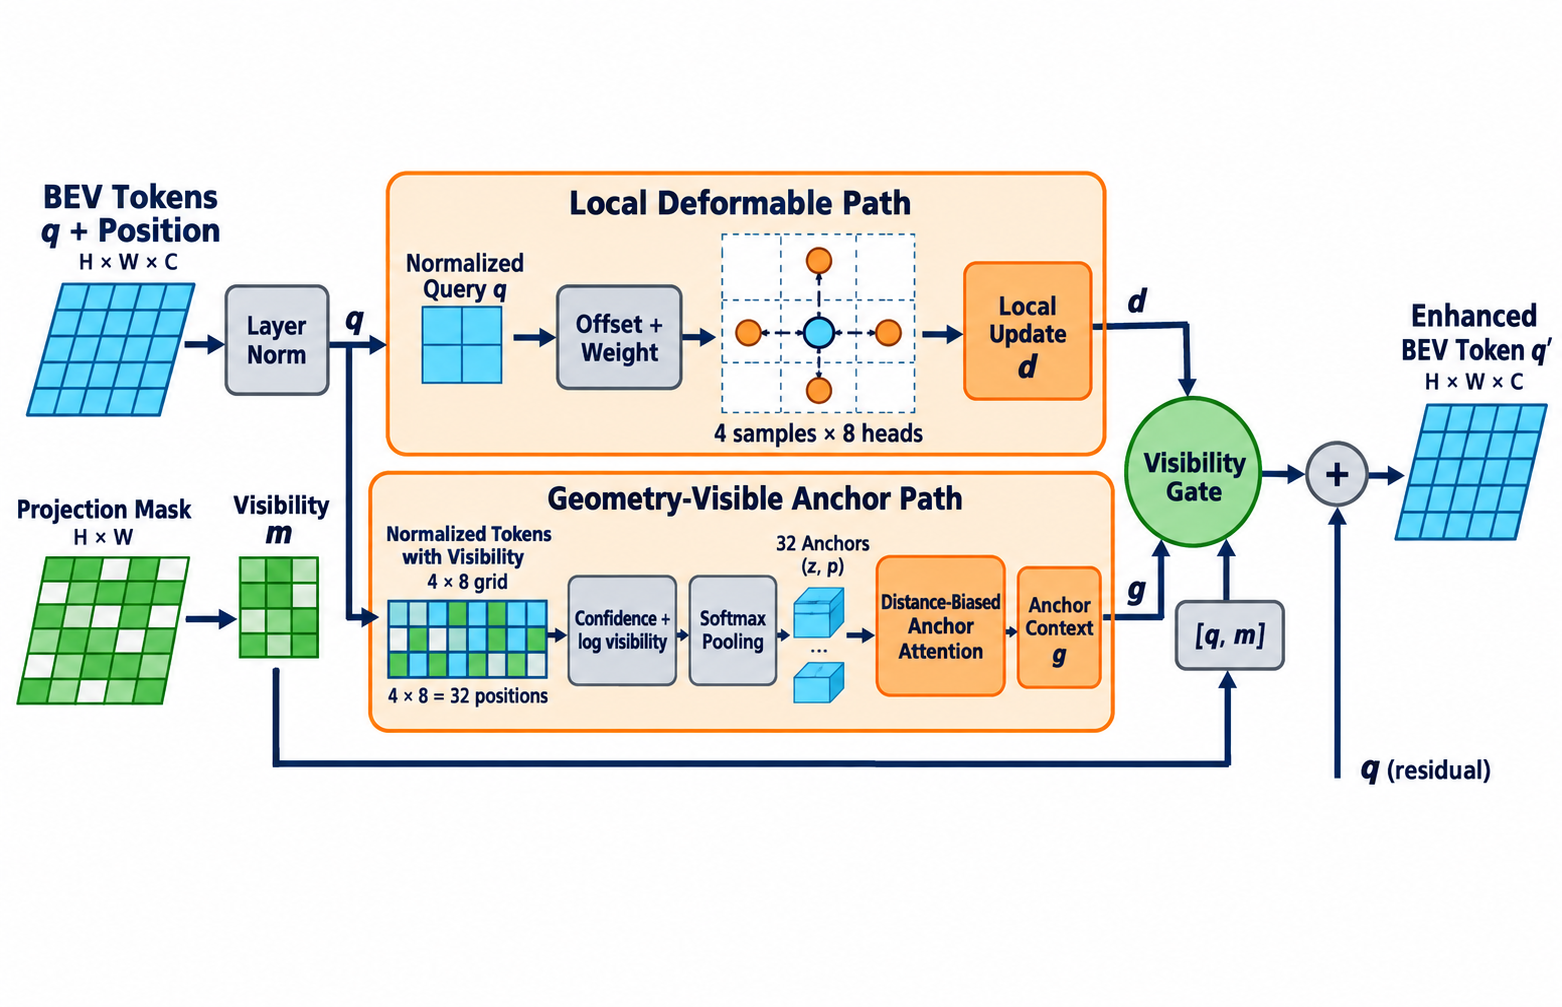
\includegraphics[width=\linewidth]{figures/gvad_detailed_architecture_v2.png}
\caption{(b) GVAD 详细架构。相机投影掩码首先归约为每个 BEV token 的可见性；局部可变形路径根据查询预测采样位置和权重，形成局部更新；几何可见锚点路径将 BEV 平面划分为 $4\times8$ 个 tile，以特征置信度和可见性加权构建 32 个锚点，并通过距离偏置的多头注意力形成锚点上下文。两条路径经可见性门控和残差连接融合为增强 BEV token。}
\label{fig:gvad}
\end{figure}

\subsubsection{近远场 BEV 查询布局}\label{sec:nearfar}
农业机器人规划与避障对近场误差尤为敏感：近处作物、垄沟和障碍物在图像中具有足够像素支持，且其细粒度几何直接决定可通行空间；远处区域的投影更小、遮挡更强，连续使用与近场相同密度的 BEV 查询却带来大量冗余计算。均匀的 $100\times100$ 查询布局没有反映这种观测质量和任务重要性的空间差异，在有限算力下同时维持全域稠密编码，会挤占本应投入近场精细结构的计算预算。因此，需要一种在不改变最终稠密占用输出的前提下，将早期编码能力优先分配给近场的查询布局。

为此，本文采用近远场 BEV 查询布局。设 BEV 宽度方向对应前向距离，将前 $60\%$ 列作为近场，保留全部查询；其余远场每隔 2 个单元在二维规则网格保留一个查询。前五个编码层只处理这些 active token。对于未激活远场位置，使用其四个相邻 active token 的双线性权重恢复特征；最后一个编码层恢复为完整 $100\times100$ 网格并执行一次稠密、图像条件的交叉注意力。该安排避免仅由查询插值补全远场语义，同时使已有占用解码头保持不变。GVAD 在稀疏层中按 token 的原始稠密 BEV 坐标分箱生成锚点，而不是把非均匀 token 序列误当作一维图像。

图\ref{fig:nearfar} 给出了近远场布局。它保留近场的完整网格以表达作物、垄沟和障碍物的细粒度几何，同时对远场执行规则稀疏采样，并在进入最终稠密图像交叉注意力前恢复完整特征图。
\begin{figure}[t]
\centering
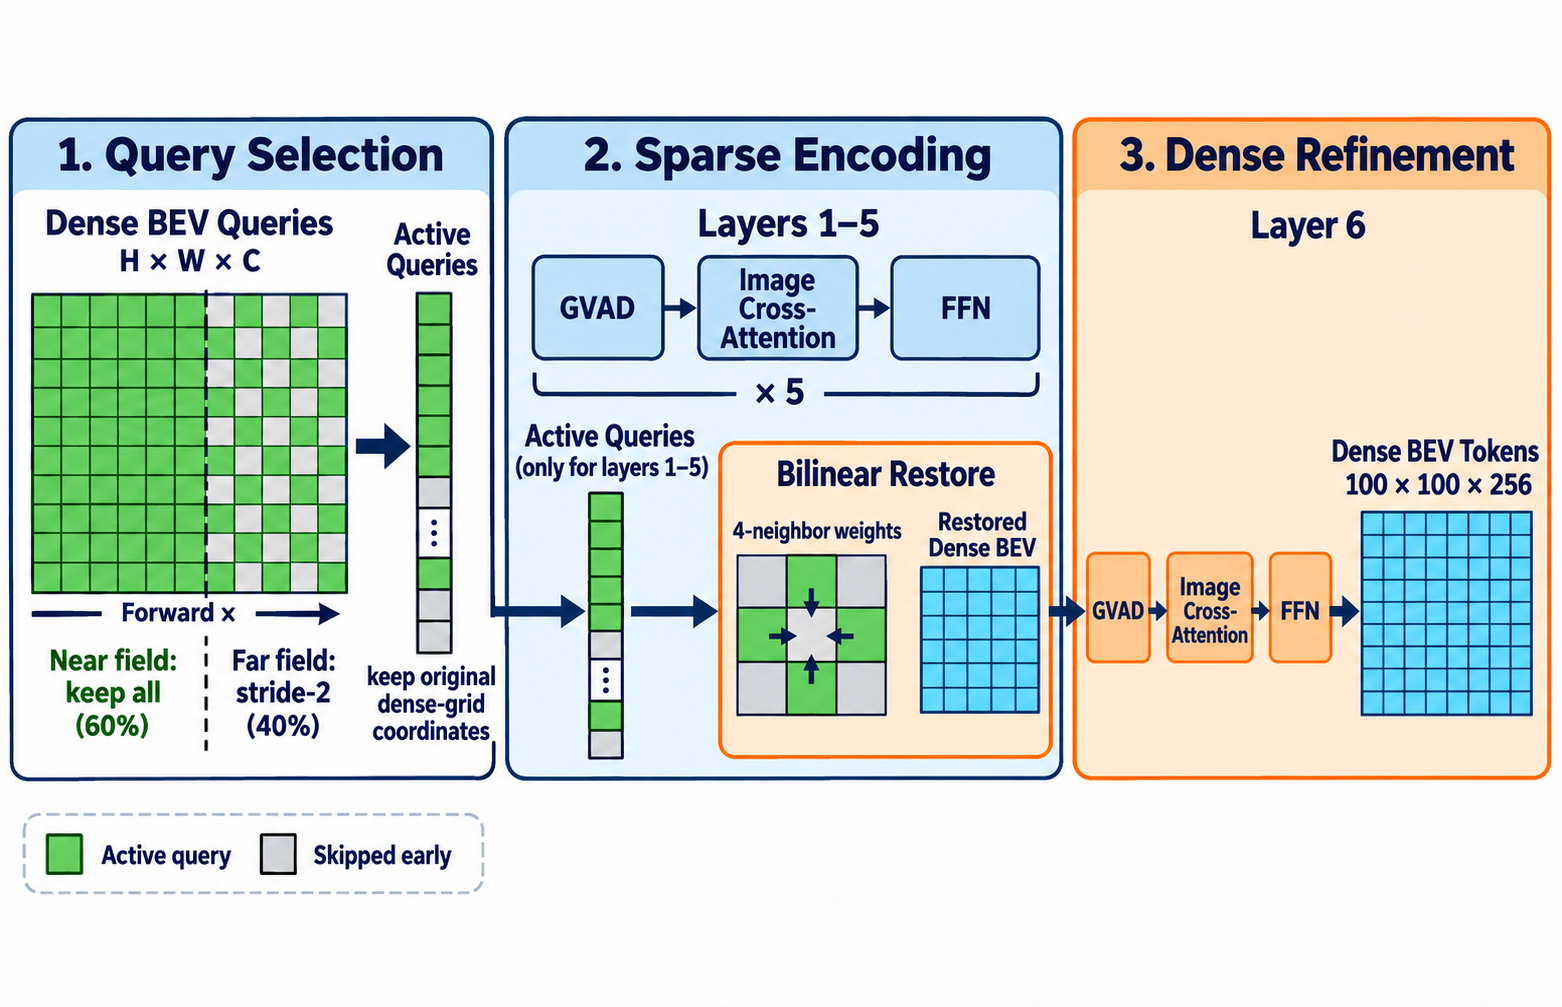
\includegraphics[width=\linewidth]{figures/nearfar_detailed_architecture_v2.png}
\caption{(c) NearFar 详细架构。输入稠密 BEV 网格沿前向距离划分为近场与远场：前 $60\%$ 的近场保留全部查询，后 $40\%$ 的远场按步长 2 规则激活。所有 active token 保留其原始稠密网格坐标，并在前五层进行稀疏编码；随后，未激活远场位置由相邻四个 active token 的双线性权重恢复为完整网格，再送入最终稠密图像条件细化层。}
\label{fig:nearfar}
\end{figure}

\subsection{农业结构自适应混合专家三维占用解码器}\label{sec:agri-amoe}
农田占用空间具有显著的各向异性：作物行与垄沟在地平面上呈现长程连续和周期性交替，
作物冠层、土壤和障碍物又在高度方向具有不同的边界形态。
特别是株间空隙和作物与自由空间的边界往往只占少量体素，
若将二维 BEV token 独立地直接映射为各高度类别，
解码器难以协调相邻位置的平面细节与垂直结构，预测容易在细粒度区域发生过度平滑。
因而，最终占用头不仅需要恢复高度维度，还应按局部三维结构的复杂度自适应地选择合适的感受野与方向建模方式。

基于这一考虑，本文设计农业结构自适应混合专家三维占用解码器（Agri-AMoE），并仅替换最终预测层的 MLP 解码。对于最终层 BEV 特征 $\bm{Q}\in\R^{B\times HW\times C}$，先经线性映射并重排为通道数为 $C_a$ 的三维体积
\begin{equation}
\bm{F}_0=\operatorname{reshape}(W_{\mathrm{lift}}\bm{Q})\in\R^{B\times C_a\times Z\times H\times W}.
\end{equation}
本文使用 $C_a=96$、$Z=25$。通道显著性由全局三维池化后的两层 $1\times1\times1$ 变换产生，并先调制体积特征；空间显著性由该特征的通道均值和最大值生成，作为路由的空间线索：
\begin{equation}
\bm{F}=\bm{F}_0\odot\sigma\!\left(f_c(\operatorname{GAP}(\bm{F}_0))\right),\qquad
\bm{S}=\sigma\!\left(f_s([\operatorname{mean}_c(\bm{F}),\operatorname{max}_c(\bm{F})])\right).
\end{equation}

为使专家选择与三维结构复杂度对齐，Agri-AMoE 计算体积特征在三个空间方向的有限差分能量：
\begin{equation}
\bm{E}=\operatorname{mean}_c\!\left((\nabla_x\bm{F})^2+(\nabla_y\bm{F})^2+(\nabla_z\bm{F})^2\right).
\end{equation}
逐体素路由器以 $[\log(1+\bm{E}),\bm{S}]$ 为输入，在温度 $\tau=1$ 下输出三个专家权重 $\bm{\alpha}=\operatorname{Softmax}(g([\log(1+\bm{E}),\bm{S}])/\tau)$。三个轻量深度可分离专家分别采用 $1\times3\times3$ 卷积编码株间平面细节、$3\times1\times1$ 卷积编码垂直结构、以及膨胀率为 2 的 $1\times3\times3$ 卷积编码较大范围平面上下文。最终的残差混合为
\begin{equation}
\bm{F}'=\operatorname{ReLU}\!\left(\bm{F}+\operatorname{GN}\!\left(\sum_{k=1}^{3}\alpha_k\mathcal{E}_k(\bm{F})\right)\right),\qquad
\bm{O}=W_o\bm{F}',
\end{equation}
其中 $W_o$ 为 $1\times1\times1$ 分类卷积，$\bm{O}\in\R^{B\times6\times Z\times H\times W}$ 为最终语义 logits。该模块在推理时参与主预测，而不是训练期辅助细化分支，因此真正改变了最终占用头读取和融合三维视觉表征的方式。

图\ref{fig:agri-amoe}以结构示意展示该解码过程：二维 BEV token 经 lifting 形成三维体积，通道/空间显著性和三方向梯度能量共同驱动逐体素路由，三个各向异性专家的输出经残差混合后用于最终分类。
\begin{figure}[t]
\centering
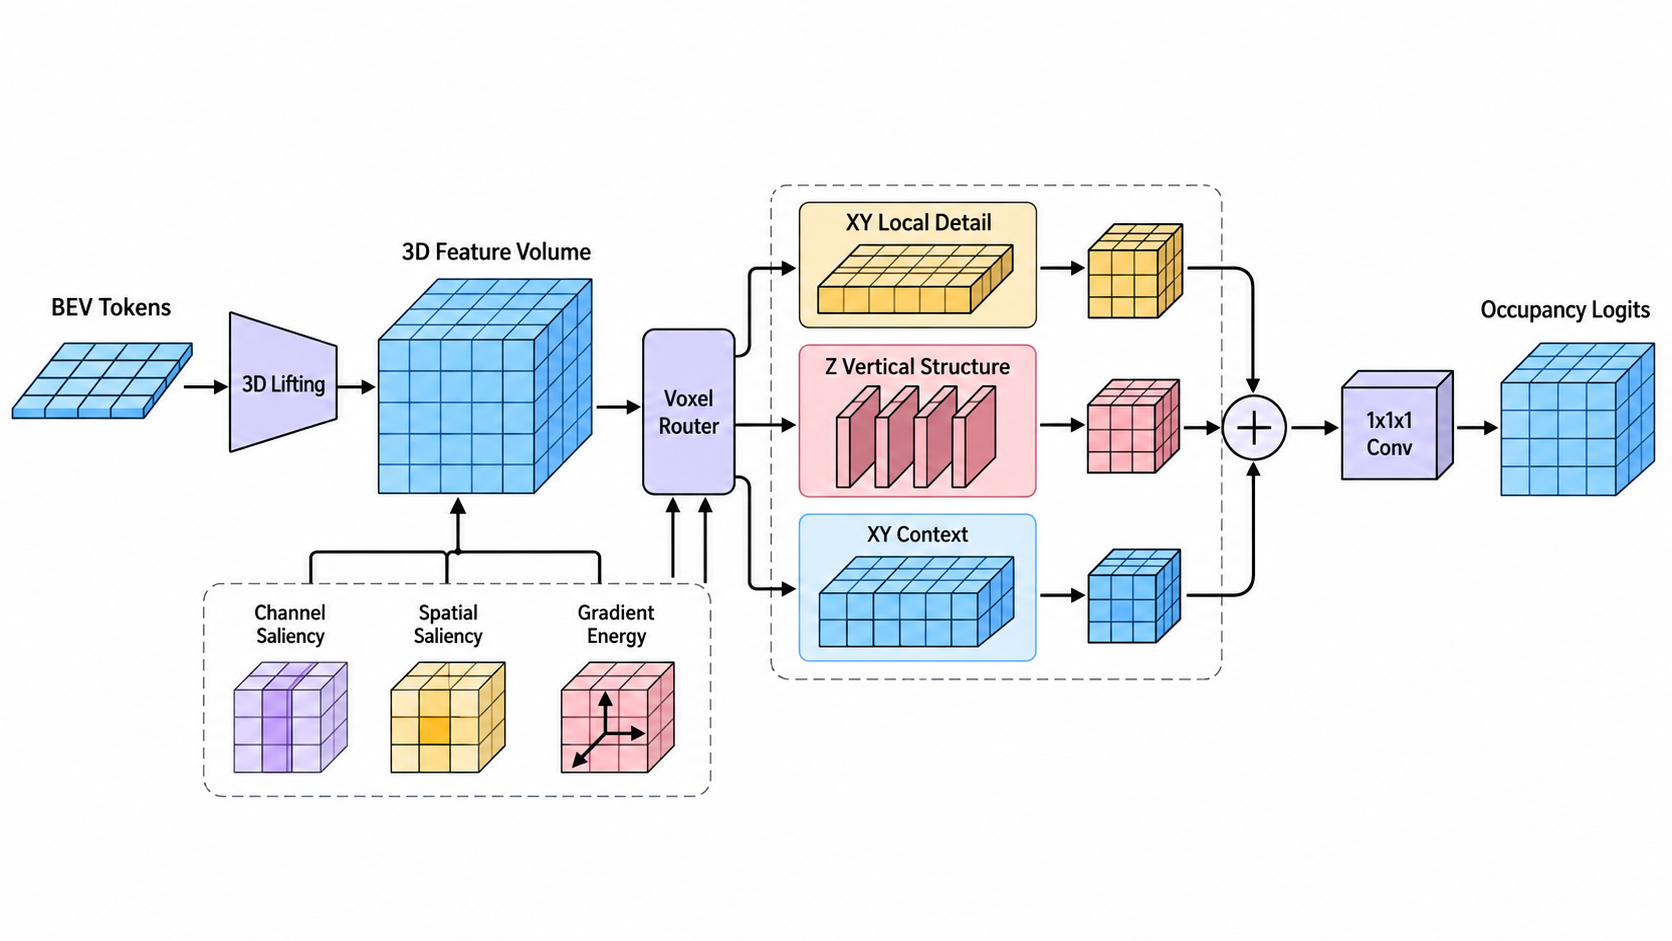
\includegraphics[width=\linewidth]{figures/agri_amoe_module_imagegen.png}
\caption{Agri-AMoE 三维占用解码器。最终 BEV token 被提升为三维特征体；通道显著性、空间显著性与 $x/y/z$ 方向梯度能量输入逐体素路由器，分别激活平面局部细节、垂直结构和大范围平面上下文专家。三个专家的加权结果经残差混合与 $1\times1\times1$ 分类卷积产生语义体素 logits。}
\label{fig:agri-amoe}
\end{figure}

\subsection{总体优化目标}\label{sec:loss}
占用主损失沿用多层解码器监督，包含类别交叉熵、语义尺度损失、几何尺度损失和 Lov\'{a}sz-Softmax 项。记该损失为 $\mathcal{L}_{\mathrm{occ}}$，则训练目标为
\begin{equation}
\mathcal{L}=\mathcal{L}_{\mathrm{occ}}.
\end{equation}
GVAD、Agri-AMoE 和近远场模块均不引入额外标签或额外损失；Agri-AMoE 通过改变最终层的预测参数化学习三维结构，而非依赖训练期专用监督。
